% =========================================================================
% fig_hd2_schur_hbcf_macrodominios.tex
% HBCF diakoptic partition of the island: 4 macro-domains + boundary cut
% Gamma (30 buses) and block structure A = diag(...) with 0.00e+00 off-block
% Dossier: TPWRS-SENI-142-2026 — data: canonical census + Schur NPZ (sealed)
% =========================================================================
\documentclass[tikz,border=12pt]{standalone}
\usepackage[T1]{fontenc}
\usepackage[utf8]{inputenc}
\usepackage{amsmath}
\usetikzlibrary{arrows.meta,positioning,calc,backgrounds,decorations.pathreplacing}
\definecolor{seniNavy}{RGB}{26,54,93}
\definecolor{seniRed}{RGB}{155,44,44}
\definecolor{seniBlue}{RGB}{43,108,176}
\definecolor{seniGold}{RGB}{190,140,40}
\definecolor{seniGreen}{RGB}{39,103,73}
\tikzset{>={Stealth[length=2.5mm,width=1.8mm]},
         lbl/.style={font=\footnotesize,align=left},
         lblS/.style={font=\scriptsize,align=left}}
\begin{document}
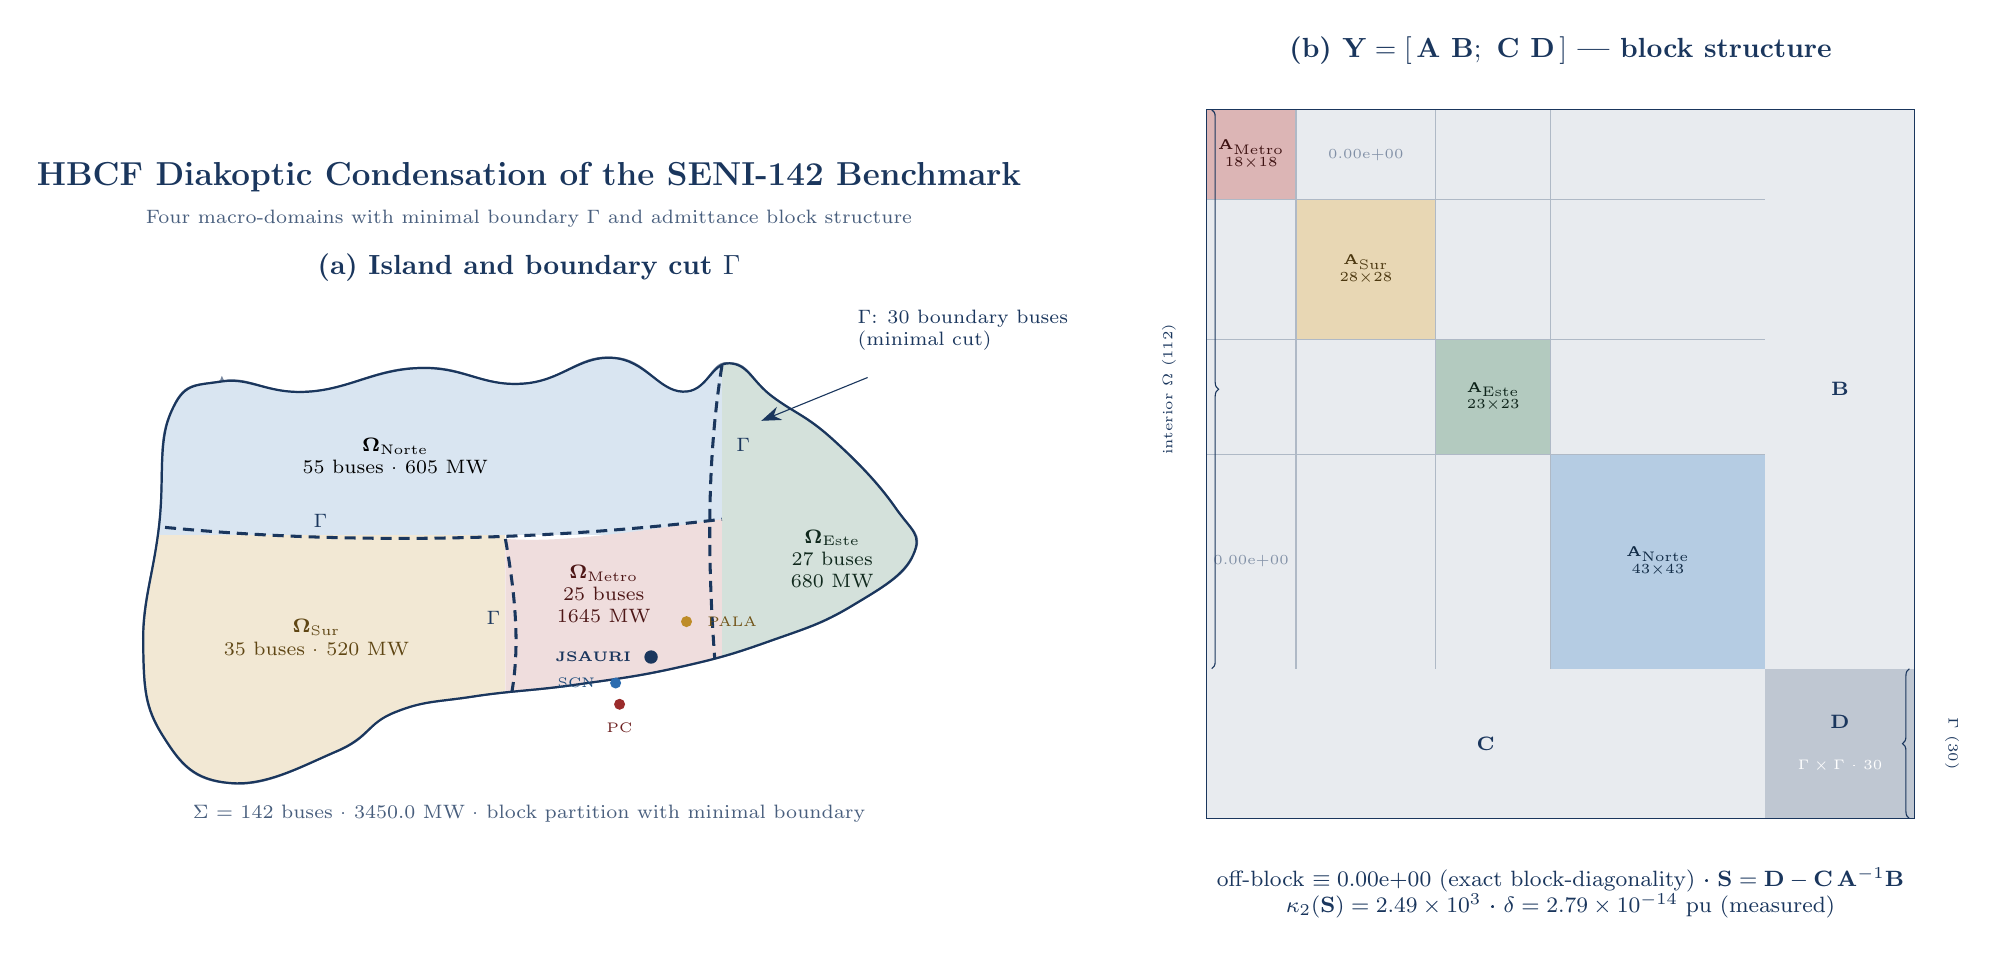
\begin{tikzpicture}[x=1cm,y=1cm]

% ================================================================= TITLE
\node[lbl,font=\large\bfseries,seniNavy] at (5.0,8.15)
  {HBCF Diakoptic Condensation of the SENI-142 Benchmark};
\node[lblS,seniNavy!80] at (5.0,7.62)
  {Four macro-domains with minimal boundary $\Gamma$ and admittance block structure};

% =======================================================================
% PANEL (a): DIAKOPTIC ISLAND MAP
% =======================================================================
\node[lbl,font=\bfseries,seniNavy] at (5.0,7.0) {(a) Island and boundary cut $\Gamma$};

% schematic island silhouette
\path[fill=white,draw=seniNavy!60,thick,rounded corners=1pt]
  plot[smooth cycle,tension=0.75] coordinates{
   (0.45,5.15) (1.10,5.55) (2.20,5.42) (3.60,5.72) (4.90,5.52)
   (6.05,5.85) (6.95,5.42) (7.55,5.78) (8.10,5.35) (8.85,4.82)
   (9.65,3.95) (9.88,3.35) (9.10,2.70) (8.05,2.25) (6.90,1.92)
   (5.60,1.70) (4.30,1.55) (3.30,1.35) (2.55,0.85) (1.20,0.45)
   (0.35,1.05) (0.10,2.20) (0.30,3.70)};
\begin{scope}
  \clip plot[smooth cycle,tension=0.75] coordinates{
   (0.45,5.15) (1.10,5.55) (2.20,5.42) (3.60,5.72) (4.90,5.52)
   (6.05,5.85) (6.95,5.42) (7.55,5.78) (8.10,5.35) (8.85,4.82)
   (9.65,3.95) (9.88,3.35) (9.10,2.70) (8.05,2.25) (6.90,1.92)
   (5.60,1.70) (4.30,1.55) (3.30,1.35) (2.55,0.85) (1.20,0.45)
   (0.35,1.05) (0.10,2.20) (0.30,3.70)};
  % fills per macro-domain
  \fill[seniGreen!20] (7.45,0.0) rectangle (10.2,7.0);   % Este (x>7.45)
  \fill[seniBlue!18]  (0.0,3.60) rectangle (7.45,7.0);   % Norte (y>3.6)
  \fill[seniRed!16]   (4.70,1.30) .. controls (5.60,1.60) and (6.40,1.65)
                      .. (7.45,1.30) -- (7.45,3.80) .. controls (6.20,3.62)
                      and (5.40,3.50) .. (4.70,3.55) -- cycle; % Metro
  \fill[seniGold!20]  (0.0,0.0) rectangle (4.70,3.60);   % Sur (remaining SW)
  % boundary cuts Gamma
  \draw[seniNavy,line width=1.1pt,dash pattern=on 4pt off 2.5pt]
    (0.15,3.72) .. controls (2.20,3.50) and (4.80,3.48) .. (7.45,3.80);
  \draw[seniNavy,line width=1.1pt,dash pattern=on 4pt off 2.5pt]
    (7.45,5.75) .. controls (7.20,4.20) and (7.30,2.60) .. (7.42,1.28);
  \draw[seniNavy,line width=1.1pt,dash pattern=on 4pt off 2.5pt]
    (4.70,3.55) .. controls (4.85,2.70) and (4.90,2.00) .. (4.72,1.32);
  \node[font=\scriptsize\bfseries,seniNavy] at (2.35,3.78) {$\Gamma$};
  \node[font=\scriptsize\bfseries,seniNavy] at (7.72,4.75) {$\Gamma$};
  \node[font=\scriptsize\bfseries,seniNavy] at (4.55,2.55) {$\Gamma$};
\end{scope}
% outline redrawn on top of the fills
\draw[seniNavy,thick] plot[smooth cycle,tension=0.75] coordinates{
   (0.45,5.15) (1.10,5.55) (2.20,5.42) (3.60,5.72) (4.90,5.52)
   (6.05,5.85) (6.95,5.42) (7.55,5.78) (8.10,5.35) (8.85,4.82)
   (9.65,3.95) (9.88,3.35) (9.10,2.70) (8.05,2.25) (6.90,1.92)
   (5.60,1.70) (4.30,1.55) (3.30,1.35) (2.55,0.85) (1.20,0.45)
   (0.35,1.05) (0.10,2.20) (0.30,3.70)};

% anchor substations of the metropolitan triangle
\fill[seniNavy] (6.55,2.05) circle (0.085);
\node[font=\tiny\bfseries,seniNavy,anchor=east] at (6.42,2.05) {JSAURI};
\fill[seniRed]   (6.15,1.45) circle (0.07);
\node[font=\tiny,seniRed!70!black,anchor=north] at (6.15,1.33) {PC};
\fill[seniGold]  (7.00,2.50) circle (0.07);
\node[font=\tiny,seniGold!60!black,anchor=west] at (7.14,2.50) {PALA};
\fill[seniBlue]  (6.10,1.72) circle (0.07);
\node[font=\tiny,seniBlue!70!black,anchor=east] at (5.96,1.72) {SCN};

% macro-domain labels
\node[lblS,align=center] at (3.30,4.60)
  {$\boldsymbol{\Omega_{\text{Norte}}}$\\ 55 buses · 605 MW};
\node[lblS,align=center,seniRed!50!black] at (5.95,2.85)
  {$\boldsymbol{\Omega_{\text{Metro}}}$\\ 25 buses\\ 1645 MW};
\node[lblS,align=center,seniGreen!40!black] at (8.85,3.30)
  {$\boldsymbol{\Omega_{\text{Este}}}$\\ 27 buses\\ 680 MW};
\node[lblS,align=center,seniGold!50!black] at (2.30,2.30)
  {$\boldsymbol{\Omega_{\text{Sur}}}$\\ 35 buses · 520 MW};

% Gamma callout
\draw[->,seniNavy] (9.30,5.60) -- (7.95,5.05);
\node[lblS,seniNavy,anchor=west,align=left] at (9.05,6.20)
  {$\Gamma$: 30 boundary buses\\ (minimal cut)};
\node[lblS,seniNavy!80,anchor=north] at (5.0,0.30)
  {$\Sigma$ = 142 buses · 3450.0 MW · block partition with minimal boundary};

% =======================================================================
% PANEL (b): BLOCK STRUCTURE  Y = [A B; C D]
% =======================================================================
\begin{scope}[shift={(13.6,0)}]
\node[lbl,font=\bfseries,seniNavy] at (4.5,9.75)
  {(b) $\mathbf{Y}=[\,\mathbf{A}\ \mathbf{B};\ \mathbf{C}\ \mathbf{D}\,]$ — block structure};

% unit: 142 rows -> 9 cm ; interiors 112 (18+28+23+43) on top, boundary 30 below
\pgfmathsetmacro{\u}{0.06338}
\pgfmathsetmacro{\wM}{18*\u} \pgfmathsetmacro{\wS}{28*\u}
\pgfmathsetmacro{\wE}{23*\u} \pgfmathsetmacro{\wN}{43*\u}
\pgfmathsetmacro{\wG}{30*\u}
\pgfmathsetmacro{\hA}{112*\u}
\pgfmathsetmacro{\yI}{\wG}          % base of the interior zone (A and B)

% B (top right), C (bottom left), D (bottom right)
\fill[seniNavy!10] (0,\yI) rectangle (\hA+\wG,\yI+\hA);
\fill[seniNavy!10] (0,0) rectangle (\hA,\wG);
\fill[seniNavy!28] (\hA,0) rectangle (\hA+\wG,\wG);
% diagonal blocks of A (top to bottom: Metro, Sur, Este, Norte)
\fill[seniRed!35]  (0,\yI+\hA-\wM) rectangle (\wM,\yI+\hA);
\fill[seniGold!35] (\wM,\yI+\hA-\wM-\wS) rectangle (\wM+\wS,\yI+\hA-\wM);
\fill[seniGreen!35](\wM+\wS,\yI+\hA-\wM-\wS-\wE) rectangle (\wM+\wS+\wE,\yI+\hA-\wM-\wS);
\fill[seniBlue!35] (\wM+\wS+\wE,\yI) rectangle (\wM+\wS+\wE+\wN,\yI+\wN);
% internal subdivisions of A
\draw[seniNavy!35] (\wM,\yI) -- (\wM,\yI+\hA);
\draw[seniNavy!35] (\wM+\wS,\yI) -- (\wM+\wS,\yI+\hA);
\draw[seniNavy!35] (\wM+\wS+\wE,\yI) -- (\wM+\wS+\wE,\yI+\hA);
\draw[seniNavy!35] (0,\yI+\wN) -- (\hA,\yI+\wN);
\draw[seniNavy!35] (0,\yI+\wN+\wE) -- (\hA,\yI+\wN+\wE);
\draw[seniNavy!35] (0,\yI+\wN+\wE+\wS) -- (\hA,\yI+\wN+\wE+\wS);
% outer frame
\draw[seniNavy] (0,0) rectangle (\hA+\wG,\yI+\hA);
% off-diagonal cells within A (genuinely empty cells)
\node[font=\tiny,seniNavy!55] at (\wM+\wS/2,\yI+\hA-\wM/2) {0.00e+00};
\node[font=\tiny,seniNavy!55] at (\wM/2,\yI+\wN/2) {0.00e+00};
% block labels
\node[font=\tiny,seniRed!40!black,align=center] at (\wM/2,\yI+\hA-\wM/2) {$\mathbf{A}_{\text{Metro}}$\\ 18$\times$18};
\node[font=\tiny,seniGold!40!black,align=center] at (\wM+\wS/2,\yI+\hA-\wM-\wS/2) {$\mathbf{A}_{\text{Sur}}$\\ 28$\times$28};
\node[font=\tiny,seniGreen!35!black,align=center] at (\wM+\wS+\wE/2,\yI+\hA-\wM-\wS-\wE/2) {$\mathbf{A}_{\text{Este}}$\\ 23$\times$23};
\node[font=\tiny,seniBlue!40!black,align=center] at (\wM+\wS+\wE+\wN/2,\yI+\wN/2) {$\mathbf{A}_{\text{Norte}}$\\ 43$\times$43};
\node[font=\scriptsize\bfseries,seniNavy] at (\hA+\wG/2,\wG/2+0.28) {$\mathbf{D}$};
\node[font=\tiny,white] at (\hA+\wG/2,\wG/2-0.28) {$\Gamma\times\Gamma$ · 30};
\node[font=\scriptsize\bfseries,seniNavy] at (\hA+\wG/2,\yI+\hA/2) {$\mathbf{B}$};
\node[font=\scriptsize\bfseries,seniNavy] at (\hA/2,\wG/2) {$\mathbf{C}$};

% braces
\draw[decorate,decoration={brace,mirror,raise=2pt},seniNavy] (0,\yI) -- (0,\yI+\hA);
\node[font=\tiny,seniNavy,rotate=90,anchor=south] at (-0.26,\yI+\hA/2) {interior $\Omega$ (112)};
\draw[decorate,decoration={brace,raise=2pt},seniNavy] (\hA+\wG,0) -- (\hA+\wG,\wG);
\node[font=\tiny,seniNavy,rotate=-90,anchor=south] at (\hA+\wG+0.26,\wG/2) {$\Gamma$ (30)};

% formulas below the block matrix
\node[lbl,anchor=north,align=center,seniNavy] at (4.5,-0.5)
  {off-block $\equiv 0.00\text{e+00}$ (exact block-diagonality) ·
   $\mathbf{S}=\mathbf{D}-\mathbf{C}\,\mathbf{A}^{-1}\mathbf{B}$\\
   $\kappa_2(\mathbf{S})=2.49\times10^{3}$ · $\delta=2.79\times10^{-14}$~pu (measured)};
\end{scope}

\end{tikzpicture}
\end{document}
